\chapter{Introducere}

%Aceasta lucrare își propune sa prezinte, din punct de vedere atât teoretic cat și practic în ce consta dezvoltarea unui algoritm de recunoaștere a obiectelor în imagini, folosind tehnici de procesare a imaginilor și învățare automata.

Prin intermediul acestei lucrări doresc sa prezint, atât din punct de vedere teoretic cat și practic, pașii necesari în dezvoltarea unui sistem de recunoaștere a obiectelor în imagini, folosind tehnici de procesare a imaginilor și învățare automata.



\section{Motivație}

Recunoașterea obiectelor este una dintre principalele aplicații ale viziunii artificiale și procesarea de imagini. 

Oamenii pot recunoaște o mulțime de obiecte într-o imagine fără sa depună prea mult efort, chiar dacă în aceste imagini obiectele prezintă variații de perspectiva, de dimensiune, sunt translatate, rotite sau chiar obstrucționate. 
Cu toate ca, de-a lungul timpului au fost studiați și dezvoltați multi algoritmi, sistemele de recunoaștere automata a obiectelor sunt încă departe de performanta unei fințe umane, chiar de cea a unui copil de numai doi ani, deci inca exista loc pentru cercetarea și dezvoltarea algoritmilor în acest domeniu.
În ciuda performantei relativ scăzute a acestor algoritmi, odată cu dezvoltarea sistemelor hardware, fapt ce a permis aplicarea unor algoritmi mult mai complicați sau au putut fi aplicați pe niște probleme de dimensiune mai mare, cererea de aplicații a crescut. 

Cateva dintre cele mai de succes aplicatii sunt: 
\begin{itemize}
	\item Sistemul de frânare automata la detecția pietonilor de pe mașinile Volvo.	
	\begin{figure}[H]
		\centering
			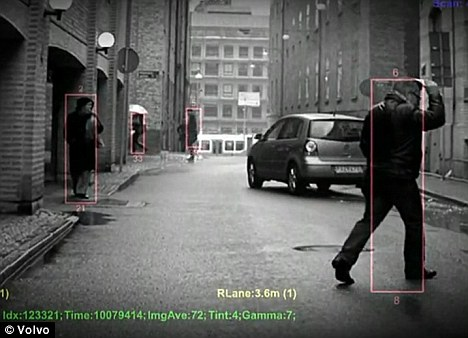
\includegraphics[width=0.9\textwidth]{imagini/volvo_pedestrian_detection.jpg}
		\caption{Volvo: sistemul de detectie a pietonilor }
		\label{fig:volvo_pedestrian_detection}
	\end{figure}	
	
	\item Focalizarea automata a camerelor foto pe fețe		
	\begin{figure}[H]
		\centering
			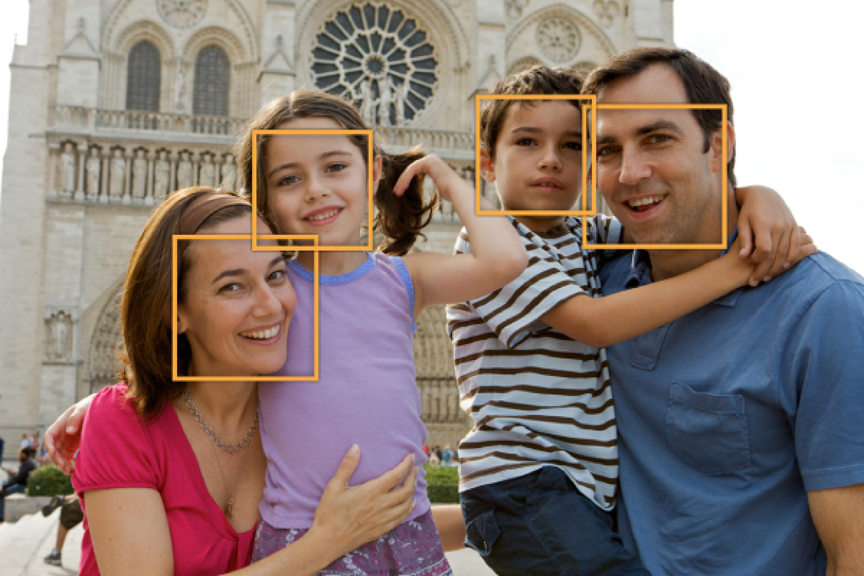
\includegraphics[width=0.9\textwidth]{imagini/face_detection_2x.png}
		\caption{Camera foto: focus automat}
		\label{fig:face_detection_2x}
	\end{figure}
	
	
	\item Analizarea traficului rutier	
	\begin{figure}[H]
		\centering
			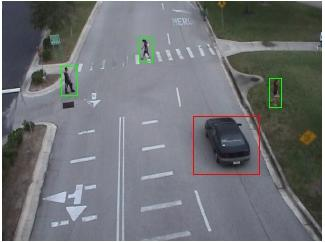
\includegraphics[width=0.9\textwidth]{imagini/traffic_analisys.jpg}
		\caption{Analizarea traficului rutier}
		\label{fig:traffic_analisys}
	\end{figure}
\end{itemize}


Înțelegerea și dezvoltarea unui sistem de recunoaștere automata a obiectelor poate fi foarte dificila, mai ales pentru cei care sunt la început de drum în studierea acestui domeniu. 
Documentația de specialitate, de cele mai multe ori, este scrisa privind problema de la un nivel foarte înalt și nu sunt tratate detaliile algoritmilor. 
În același timp, în foarte multe lucrări se fac referiri la lucrări anterioare, unele chiar cu zeci de ani distanta intre ele, acestea find uneori foarte greu de găsit.
Parcurgerea unui astfel de document, presupune cunoștințe extensive de matematica, statistica, învățare automata, procesarea imaginilor și chiar cunoștințe din domeniul biologic sau medical. 
Toate acestea fac ca nivelul de la care se intra acest domeniu sa fie unul foarte înalt, ceea ce poate fi descurajant pentru un începător.

Exista câteva librarii software bune, open-source, cu care se pot dezvolta aplicații. 
Acestea conțin algoritmi de recunoaștere a obiectelor gata implementați. 
Totuși componentele care stau la baza acestor implementări nu sunt expuse, reutilizarea lor find imposibila.
Nici codul sursa nu este ușor de urmări, acești algoritm sunt optimizați cu instrucțiuni de asamblare, cod pe mai multe fire de execuție și chiar cod care se executa pe procesorul grafic.
Din aceasta cauza, consider ca nu sunt foarte utile celor care doresc sa dezvolte sau sa implementeze algoritmi.

Doresc, ca la finalul acestei lucrări, sa obțin o platforma de dezvoltare a algoritmilor pentru recunoașterea obiectelor, pe care sa o pot folosi în activitatea mea din domeniu.
Totodată aceasta sa servească ca un punct de plecare pentru cei care doresc sa se inițieze în domeniu.

%Viziunea artificiala reprezinta procesul invers al celui de formare a imagini și se ocupa cu recuperarea de informații din imagini cu ajutorul metodelor matematice, geometrice, statistice și a teoriei învățării automate\footnote{Machine learning}.

%Recunoașterea automata a obiectelor se refera la capacitatea unui sistem software de localizare și identificare a obiectelor într-o imagine sau o secventa video.

%Din punct de vedere practic, aceasta lucrare își propune dezvoltarea unei biblioteci software și aplicații demonstrative, cu ajutorul cărora sa se poată dezvolta aplicații de recunoașterea obiectelor în imagini.

%Din punct de vedere teoretic sunt descrise componentele și structura unui astfel algoritm, precum și cel folosit pentru al antrena.



%Viziunea artificiala și învățarea automata sunt doua domenii aflate în plina dezvoltare și sunt de mare interes atât în cadrul academic ca și în industria software.

%Dezvoltarea rapida a sistemelor de calcul a permis utilizarea acestor algoritmi în tot mai multe aplicații. Câteva dintre aplicațiile recunoașterii de obiecte sunt:
%\begin{itemize}
%	\item Industriale: recunoașterea și verificarea cip-urilor pe o placa electronica, numărarea de obiecte pe o banda rulanta
%	\item Securitate: recunoașterea unui intrus folosind o camera de supraveghere
%	\item Medicale: recunoașterea diferitelor tumori într-o imagine de tomografie
%	\item Fotografie: focalizare automata pe fete
%	\item Internet: căutare google după imagini, marcarea automata a fetelor într-o poza de pe facebook
%\end{itemize}

%Interesul 

%Pana acum am folosit și am studiat o mulțime de algoritmi de recunoaștere a obiectelor, dar pentru a aprofunda înțelegerea acestor algoritmi cel mai bine este sa fie scris măcar unul de la un capăt la altul.

%Cei mai multi algoritmi de recunoaștere a obiectelor au o structura comuna formata din următoarele componente: scanarea imaginii, extragerea de trasaturi, classificare si procesarea rezultatelor.

%Multi algoritmi sunt scrisi intr-un mod foarte rigid si componentele lor nu pot fi refolosite. Sunt optimizati pana la punctul in care codul sursa nu mai poate fi inteles cu usurinta.

%In cadrul companiei la care lucrez, Dynamic Ventures, am folosi

%Desi, am folosit si m-am documentat 

%Am ales sa dezvolt o astfel de librarie, chiar daca exista si altele, din doua motive.





%Aceasta problema nu poate fi nici pe departe considerata rezolvata, de-a lungul timpului un număr mare de algoritmi au fost propuși.

%Mult timp recunoașterea automata a obiectelor în imagini a fost considera impracticabila datorita complexității de timp și spațiu a acestor algoritmi.






\section{Enunțul problemei}
Se scrie o librărie software cu ajutorul căreia sa se dezvolte algoritmi și aplicații de recunoaștere a obiectelor.

Aceasta biblioteca va fi scrisa într-un mod hibrid, cu componente implementate atât în C++ cat și în Python.

Toate componentele bibliotecii vor suporta serializare, pentru a putea fi salvate pe disc, baze de data sau trimise prin rețea în cazul unor programe distribuite.

Algoritmul va învață sa recunoască obiecte folosindu-se de un set de imagini cu exemple pozitive adnotate și exemple negative, imagini care nu conțin obiectul pe care dorim sa-l învățam.

Se scrie o aplicate care antrenează un algoritm de recunoaștere și salvează modelul învățat pe disc și o alta aplicație care încarcă modelul și îl aplica pe o imagine data.

\pagebreak
\section{Tehnologii folosite}

\subsubsection{Limbajul C++}
[Am rezervat o pagina]
\pagebreak


%Limbajul C++ este un limbaj de programare general care și este compilat în cod-mașina.
%Este un limbaj multi-paradigma, cu verificare statica a tipurilor. 
%Suporta programarea procedurala, orientata pe obiecte și generica.
%Limbajul oferă facilitați de manipulare a memoriei la nivel scăzut.
%find proiectat inițial ca un limbaj pentru programarea de sisteme(sisteme integrate, kernel sisteme de operare), performața și eficienta sunt trăsături principale.

%Dat find faptul ca este și compatibil cu limbajul C, utilizatorii C++ au la dispoziție o gama larga de librarii software din cele mai diverse ramuri de aplicații de care se pot folosii.

\subsubsection{Limbajul Python}
[Am rezervat o pagina]
\pagebreak


%\subsubsection{Limbajele C++ și Python}

%Am ales sa combin aceste doua limbaje de programare care, chiar dacă sunt foarte diferite din multe puncte de vedere, se complementează intre ele foarte bine.

%Fiecare limbaj are avantajele și dezavantajele lui.





%Pentru realizarea lucrării am ales sa folosesc C++ și Python din mai multe motive:

%C++ și Python sunt doua limbaje de programare atât de diferite încât putem spune ca se afla în capete diferite ale axei limbajelor de programare.
%\begin{itemize}
%	\item C++ este compilat în cod-mașina, Python este interpretat
%	\item Python are sistemul de tipuri dinamic și este recunoscut pentru flexibilitate
%	\item C++ are sistemul de tipuri static și este recunoscut pentru eficienta
%	\item Python eliberează automat memoria
%\end{itemize}

%Pentru multi programatori, aceste diferențe înseamna ca cele doua limbaje se complementează perfect.

%\subsubsection{Librăria OpenCV}

%Librăria OpenCV este cea mai populara librărie de procesare de imagini


\subsubsection{Librăria Boost}
[Am rezervat o pagina]
\pagebreak


\subsubsection{Librăria scikit-learn}
[Am rezervat o pagina]
\pagebreak


\subsubsection{Librăria Qt}
[Am rezervat o pagina]
\pagebreak

\section{Structura Lucrării}
Capitolele care urmează vor trata algoritmul de recunoaștere a obiectelor din punct de vedere teoretic și se va prezenta implementarea unui astfel de algoritm.

Capitolul 1 prezintă enunțul problemei și motivația acesteia

Capitolul 2 se prezintă problema generala a unui algoritm de recunoaștere.
Vor fi prezentate în detaliu componentele din structura algoritmului.
Se va prezenta o tehnica eficienta de antrenare a acestor algoritmi.

Capitolul 3 se prezintă în detaliu implementarea unei librarii de dezvoltare a algoritmilor de recunoaștere a obiectelor.

Capitolul 4 prezintă un manual de utilizare pentru aplicația de recunoaștere a obiectelor.

Capitolul 5 prezintă concluzii despre lucrare, precum și posibilități de dezvoltare.

\pagebreak